\documentclass[12pt]{scrartcl}

\include{amsfonts,amssymb,amsmath,amsthm,txfonts,pxfonts,mathrsfs,enumitem}
\usepackage[headheight=15pt,paperwidth=8.5in, paperheight=11in,margin=0.75in]{geometry}
\usepackage{lastpage}
\usepackage{fancyhdr}
\usepackage{graphicx}
\usepackage{wrapfig}
\usepackage{subfig}
\usepackage{float}

\usepackage{mathtools}
\DeclarePairedDelimiter\floor{\lfloor}{\rfloor}
\newcommand{\argmax}{\mathop{\mathrm{argmax}}} 
\newcommand{\argmin}{\mathop{\mathrm{argmin}}} 

\newcounter{teamnumb}
\setcounter{teamnumb}{54301}

\ttfamily{
\lhead{Team\ \# \theteamnumb}\rhead{Page \thepage\ of \pageref{LastPage}}}
\cfoot{}
\renewcommand{\headrulewidth}{0pt}
\pagestyle{fancy}

\title{\vspace{-1.7cm} GoodGrant Foundation: \\Next Generation Investing }
\subtitle{A Model for Post-Secondary Educational Grants\vspace{-1.3cm}}

\begin{document}
\maketitle
\thispagestyle{fancy}

\section*{Summary}
	\ \ These are the strategies of the consulting firm Team \#54301. It's five-year mission: to explore new ranking systems; to seek out new return on investments and new student performance metrics; to boldly go where no charity has gone before.\\
	
	\ \ Our strategy lies in finding the schools that are most beneficial to individual students. We recognize that the goal of students, when choosing a university is to find the best institution that would reduce their chances at poverty. We start by developing a metric for the level of alleviation of poverty caused by each university, we call it PES. We use this as the benchmark for the initial ranking of schools.\\ 

	\ \ Once that is achieved, we use the kNN algorithm to create a list of institutions that are closest in structure to our selected benchmarks. This generated list of institutions would derive the largest benefit with an increase in funding. The main goal is to improve the well-being of future generations thus our proposed conceptual return of investment is the institutions' effect on reducing poverty.  A linear maximization algorithm is applied to determine donation amount, number of students positively affected and their respective institution. \\
	
At the end of the report, we provide a list of schools selected from a subset of the U.S. National Center on Education Statistics and College Scorecard given data set. Our methods allows for the selection of fixed number of schools as well as a unique way of allowing the model to choose the number of schools that should be invested. \\
\newpage
\tableofcontents
\newpage
	

\section{Introduction}
	\subsection{The Problem}
		The Goodgrant Foundation is a charitable organization with a mission to improve educational performance of students attending colleges and universities in the United States. The foundation intends to donate a total of 100,000,000 USD to a group of schools each year, for five years. They also wish to avoid investing in universities that have already received grants from major charitable organizations such as the Gates and Lumina Foundation.\\
		
		We present a mathematical model to outline an ranking and investment strategy to provide the maximal return on investment(ROI) appropriate for an education charity.  The model is split into two sections and is applicable in choosing $1\cdots N$ institutions. \\

The first section outlines determining bench mark points and comparing the rest of the institutions to them via a k-Nearest Neighbours(kNN) Algorithm. In the second section, we derive a ROI measuring the effect the grant would have on improving student performance. In particular, our ROI reflects changes in terms of incoming poverty and outgoing poverty. In the Model Testing section, we input a subset of the U.S. National Center on Education Statistics data set and College Scorecard data set and output a list of $1,\cdots{N}$ schools, the investment amount, and number of students affected. In Sensitivity Analysis, we restrict the distance in the kNN algorithm to obtain a subset of our prioritized schools and assess the model's stability. Lastly, we summarize the findings of the paper and suggest future additions. 
	
	\subsection{Assumptions and Rationale/Justification}
	\begin{itemize}
		\item \textbf{The Gates Foundation and Lumina Foundation will continue to donate to the same school for at least two years:} Typically large charities often donate sums over the course of number years to allow highest impact. \cite{Conkey} We are able to remove those particular schools from our candidate list to avoid duplicating the two foundation efforts. 
				
		\item \textbf{Students that attend GoodGrant Grant Recipients will continue to graduation.:}  Lack of financial support is the leading cause of students dropping out of institutions. Students who receive grants have less financial stress and can focus on graduating.\cite{Trom}
		
		\item \textbf{Attainment of higher education improves poverty rates} According to the US Census Bureau, individuals with an advance degree earn on average \$72,824 per year which is significantly higher then individuals with a high school degree at \$45,400.\cite{dis} Generally, attending post-secondary education lifts individuals above the poverty-line. 

	\end{itemize}
	
	\subsection{Summary of our Approach}
		\begin{itemize}
		\item Create a benchmark setting: top 10 schools for each degree type school, that we consider to have good performance. Each school represent a class.  
		\item Identify universities that have similar characteristics to the benchmark list. 
		\item Prioritize universities to be invested in by the amount of grants they received from other sources.
		\item Determine the amount of investment and allocation to maximize the return on investment. 
		\end{itemize}
				 
\section{Model Design and Approach}
	\subsection{Notations and Definitions}
	\begin{enumerate}
		\item $U_j^{[i]} = $ university $j$ of class $i$
		\item $U_o^{[i]} = $ benchmark university for class $i$
		\item $A_j^{[i]} = $ amount invested in university $j$ for class $i$
		\item $T_j^{[i]} = $ Tuition in university $j$ for class $i$
		\item $n_j^{[i]} = $ number of students receving our grant in university $j$ for class $i$
		\item $IP_j^{[i]} = $ poverty rate of students entering university $j$ for class $i$
		\item $OP_j^{[i]} = $ poverty rate of students exiting university $j$ for class $i$
		\item $\phi_j^{[i]} = $ number of students in university $j$ for class $i$
		\item $\Phi = $ Total number of universities
		\item $g_j^{[i]} = $ maximum amout of grants to be given to university $j$ for class $i$
		\item \underline{Group}, refers to the Carnegie Classification of the university
		\item \underline{Class}, refers to which benchmark within the group, the university is closest to.
	\end{enumerate}
	
	\subsection{Benchmark Selection}
		First we omitted any below medium size universities or communal universities such as racial or religious schools. Then we partition all universities by number of years required for graduation. Lastly, we rank the universities by the amount of their poverty alleviation standards (PES), this is done based on the result and recommendation of Trombitas \cite{Trom} and College-Score Card \cite{US}.\\ 
		\begin{align}
			R_j^{[i]}=\frac{IP_j^{[i]}-OP_j^{[i]}}{IP_j^{[i]}}
		\end{align}
		Next we choose the top, highest ranking universities per `years of graduation'-group. We set these chosen universities as our benchmarks for each class in each group.\\
		i.e.
		$$
			o^{[i]} = \argmax_{j} R_j^{[i]}
		$$
		Where $o$, is to represent the benchmark index of the class $i$.

	\subsection{Categorizing Institutions into Classes}
		We aim to classify each university into some class $i$. This is done via the kNN algorithm: a non-parametric method used in classification supervised learning problems. The output is determined by a majority vote, where the object is assigned to the class most common with it's neighbors. \cite{Hastie}\\
		We set up the following model:
		Assuming $j\in [1,n]$,where $n$ = amount of variables. For a detailed selection list please see Appendix 1. Let $y_j^{[i]}$ be the $j$-th variable for the $i$-th class benchmark. Let $x_j$ be the $j$-th variable of a particular university. A university $u$, is considered a member of the $k$-th class if the variables $x_i$ of that university is `close' to a particular variable of a given class in euclidean-space.\\
	
		That is, if $u$ belongs to the $k$-th class then
		$$
			k = \argmin_{i} \sqrt{ \sum_{j=1}^n (x_j-y_j^{[i]})^2 }
		$$

	
	\subsection{Investment Strategy}

	\subsubsection{Number of students-Helped}
		Let $A_j^{[i]}$ be the amount we invest in university $j$ of the class $i$, and $T_j^{[i]}$ be the tuition of low-income students. Then we can compute the number of students who we help as:
		\begin{align}
			n_j^{[i]} &= \floor{\frac{A_j^{[i]}}{T_j^{[i]}}}
		\end{align}

	\subsubsection{Adjusted Poverty}
		Next we computed the adjusted poverty rate. We make a crucial assumption here about the correlation between grant-money and retention rates. We assume that every student who receive the grant will stay in the program and university (this assumption can be adjusted by a future study on the probabilities between grant and retention rates).\\
		\\
		Let $\phi_j^{[i]}$ be the total number of students in university $j$ for class $i$.\\
		The adjusted rate of existing poor students based on our assumptions is:
		\begin{equation}
			OP_j^{[i]*} = \frac{  OP_j^{[i]}\phi_j^{[i]}-n_j^{[i]}  }{ \phi_j^{[i]}  }
		\end{equation}
		
		We can then provide a rank to this university, in the similar fashion we computed the rank for the benchmark universities (recall eq. (1)):
		$$
			R_j^{[i]*}=\frac{IP_j^{[i]}-OP_j^{[i]*}}{IP_j^{[i]}}
		$$
		We use this to compute the increase to the social well-being of students going to this university. 

	\subsubsection{Return on Investment (ROI)}
		The return on investment for our model will be the change in the level of alleviation of poverty provided by our investment.\\
		We do this as follows:
		\begin{equation}
			R_j^{[i]}(1+r_j^{[i]}) = R_j^{[i]*}
		\end{equation}
		where $r_j^{[i]}$ is the return on investment for a particular school.\\
		We also note that (4) can be rewritten using (1) and (3):
		\begin{equation}
			r_j^{[i]} = \frac{ OP_j^{[i]} - OP_j^{[i]*}  }{ IP_j^{[i]} - OP_j^{[i]}  }
		\end{equation}	
	 	This will later be used for simplification purpose of the maximization problem.\\
		\\
		We then average these rates, to get the approximated return:
		\begin{equation}
			\bar{r} = \frac{ \sum_{j=1}^\infty\sum_{i=1}^\infty r_j^{[i]}  }{ \Phi }
		\end{equation}
		Where $\Phi$ is the total number universities.
		

	\subsubsection{Maximization of return}
		Now that we have a measure of return on investment, we wish to maximize this measure based on the physical restriction that are given to us.\\
		Since we only have a limit of \$$100$M, and would not want to overshoot our investment by giving any particular university more than what the top-tier schools are given. We put the following restriction forth.\\
		\\
		Where $g_j^{[i]} = \max( \frac{  G_o^{[i]}  }{  \phi_o^{[i]} } - \frac{  G_j^{[i]}  }{  \phi_j^{[i]} } \ ,\ 0 )$, is the difference between per student investment with the benchmark school. We formulate the problem as follows:
		\begin{equation}
				\begin{aligned}
					& \underset{A}{\text{maximize}}
					& &\bar{r}\\
					& \text{subject to}
					& & \sum \sum A_j^{[i]} = 100,000,000 \\
					&&& \forall i,j \ \ \ 0\le A_j^{[i]} \le g_j^{[i]}\phi_j^{[i]}
				\end{aligned}
		\end{equation}

	\subsubsection{Simplifying the complexity}
		In order to simplify the complexity of the previous problem we outlined before. We reformulated the problem as follows:\\
		First, we rewrote (5) using (2) as,
		\begin{equation}
			\begin{aligned}
			r_j^{[i]} &= \frac{1 }{ \phi_j^{[i]} (IP_j^{[i]} - OP_j^{[i]} ) } n_j^{[i]}\\ 
			r_j^{[i]} &= \Delta_j^{[i]} n_j^{[i]}
			\end{aligned}
		\end{equation}	
		We note that $\Delta_j^{[i]}$ from (4) is the information given by our data. It must be positive as $$\Delta_j^{[i]}\implies IP_j^{[i]} < OP_j^{[i]}$$
		Which means that the considered university is getting more in funding than the benchmark one. If this happens, we omit that university from our dataset.\\ 
		\\
		Whereas $n_j^{[i]}$ is the number of students we invest in, which is a variable that will be controlled by us.\\
		\\
		Hence the problem as outlined in (6) return can be written as:
		\begin{align}
			\bar{r} &= \sum_{j=1}^\infty\sum_{i=1}^\infty \frac{ 1  }{ \Phi } r_j^{[i]} = \frac{ 1  }{ \Phi }\sum_{j=1}^\infty\sum_{i=1}^\infty \Delta_j^{[i]}n_j^{[i]}
		\end{align}
		So our new maximization problem can be reformulated as follows:
		\begin{equation}
				\begin{aligned}
					& \underset{\forall n_j^{[i]}}{\text{maximize}}
					& &\frac{ 1  }{ \Phi }\sum_{j=1}^\infty\sum_{i=1}^\infty \Delta_j^{[i]}n_j^{[i]}\\
					& \text{subject to}
					& & \sum \sum n_j^{[i]}T_j^{[i]} = 100,000,000\\
					&&& \forall i,j \ \ \ 0\le n_j^{[i]} \le \frac{g_j^{[i]}\phi_j^{[i]}}{T_j^{[i]}}
				\end{aligned}	
		\end{equation}
	\subsection{Limiting Schools}
		The model outlined in the previous section, is given the ability to reject schools. This can be seen in the condition:
		\begin{align*}
			\forall i,j \ \ 0\le n_j^{[i]} \le \frac{g_j^{[i]}\phi_j^{[i]}}{T_j^{[i]}}
		\end{align*}
		However, we wanted to eliminate this ability, in order to provide the capacity to maximize over any number of schools. So we reworte te condition as 
		\begin{align}
			\forall i,j \ \ 1\le n_j^{[i]}T_j^{[i]} \le g_j^{[i]}\phi_j^{[i]}
		\end{align}	
		As a side note, this would mean that $g_j^{[i]}\phi_j^{[i]}\ge1$. Meaning, that some schools may be omitted before the optimization process starts.
\section{Model Application} 
	\subsection{Partitioning and Benchmark}
		As discussed in the previous section, the first goal in the analysis is to find a list of benchmark schools. However, before doing so, we partitioned the schools by the type of degrees that they predominantly provide. This was due to the fact that otherwise, many pieces of data become unusable, and the kNN algorithm becomes biased towards schools that have less-years-to-graduation.\\ 
		\\
		Once we acquired this data, we chose the top 10 schools from each school type as our benchmark schools. It is also important to note the schools here do not \underline{only} provide the designated degree, but rather have a predominate focus on such degrees.\\
		\begin{figure}[H]
		\centering
			\subfloat[2 Year Program]{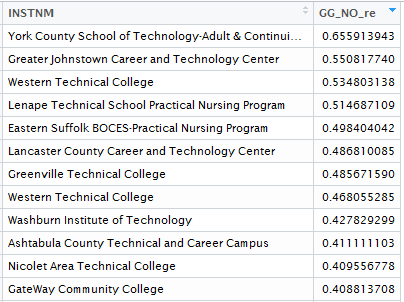
\includegraphics[width=0.45\textwidth]{2yr-col.png}}
		\qquad
			\subfloat[Bachelor Program]{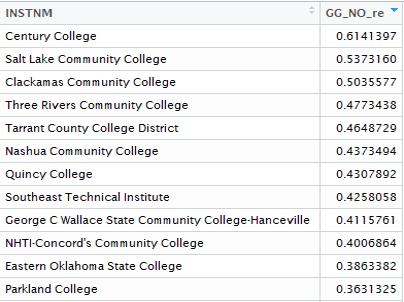
\includegraphics[width=0.465\textwidth]{4yr-col.png}}
		\end{figure}
		
		\begin{wrapfigure}{l}{0.50\textwidth}
		\centering
		\includegraphics*[width=0.90\linewidth]{6yr-col.png}\caption*{(c) 6 Year Program}
		\end{wrapfigure} 	
		We used the schools noted in Figures (a),(b) and (c) as our benchmark schools for the kNN method. These school already preform well based on our ranking, and we wanted to find the next best schools that would benefit from an investment by our charity.
		\\
		\\
		\\
		\\
		\\
		\\
		\\
		\\
		\\
	\subsection{Variable Selection}
		\subsubsection{Filtering by Grant}
			\ \ Since we did not want to overlap with grants given by other institutions, we filtered the next list using the data given by the Gates \cite{Bill} and Lumina \cite{Grant} Foundations. We did this by simply omitting schools that passed a particular threshold we set.
		
		\subsubsection{Scorecard Variables}
			\ \ Since not all the variables in the provided dictionary were given to us. We first we created a dictionary for all the variables that were given to us by Scorecard. We did this by comparing the variable titles in the dictionary and the data. \\
			
			\ \ Then we categorized these variables as follows:
			\begin{itemize}
				\item \textbf{Irrelevant [0]}, values such as location of website, or miscellaneous ids.
				\item \textbf{Informative [1]}, flags for women-only, historically black colleges and others. 
				\item \textbf{Selected [2]}, the values we chose to focus on, such as SAT, ACT, retention rates, graduation rates, tuition, debt of completers and income of students after graduation. 
				\item \textbf{Percentile [3]} values that refer to the composition of the student body (such as racial, sexual or income composition).
			\end{itemize}
			\ \ We did make use of [1], and [3], for cleaning and producing other variables (such as the PES rank), however we did not run the kNN algorithm on them.

<<<<<<< HEAD
		\subsubsection{Selection of Variables from Given Data Sets}
			Since many of the variables provided by scorecard, overlapped with the ones from IPEDS, we only withdrew the following variables:
=======
		\subsubsection{IPEDS Variables}
			\ \ Since many of the variables provided by scorecard, overlapped with the ones from IPEDS, we only withdrew the following variables:
>>>>>>> 7aaef66ef6db70fa7702596e037c20396930e9b0
			\begin{itemize}
				\item \textbf{Number of students}, which we used for computation of kNN and for the maximization algorithm.
				\item \textbf{Average Tuition of Low Income Students}, which we used mainly for the maximization.
				\item \textbf{Faculty to Student ratio}, used only for the maximization.
				\item \textbf{Total Grants Received}, we summed the various grants that each university received to get this number. We then used it for both kNN and maximization.
			\end{itemize}
	
	\subsection{kNN Selection}
		\ \ After this point, we used the kNN algorithm as the method of selection for the nearest best schools. As we wish to avoid investing in the top tier schools, and would rather invest in schools with the potential to become the top-tier. \\

		\ \ Prior to the application of the kNN algorithm we normalized the data by transforming each variable to a scale in $[0,1]$, in order to avoid bias for larger scaled-values.\\
		\clearpage
		\ \ This identification provided us with the following schools as can be seen in fig.\ref{fig:kNN}.
		\begin{figure}[H]
			\centering
			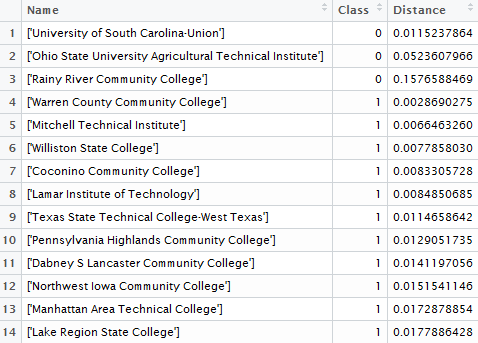
\includegraphics[width=0.45\textwidth]{nearest-schools.png}
			\caption{Sample of kNN results}
			\label{fig:kNN}
		\end{figure}
		(please note that this is not the entire dataset).
	
	\subsection{Maximizing the Return}
		\ \ Since our ultimate goal is to invest in schools that would offset poverty the most. We focused on the change in PES. The amount invested in each school should therefore maximize the increase in PES. This increase is our measurement for ROI.\\
		
		\ \ The set up for this problem is outlined in sections 2.4-2.5, using equations (10) and (11) and the aggregation of all the school's variables into a single list we can get the following:
		\begin{equation*}
				\begin{aligned}
					& \underset{\forall n_j}{\text{maximize}}
					& &\frac{ 1  }{ \Phi }\sum_{j=1}^\Phi \Delta_j n_j\\
					& \text{subject to}
					& & \sum_{j=1}^\Phi n_j\cdot T_j = 100,000,000\\
					&&& \forall i,j \ \ \ 1\le n_j\cdot T_j \le g_j\phi_j
				\end{aligned}	
		\end{equation*}

		\ \ We used the linear-optimization method described in Winston \cite{Winston}, in order to solve this problem. Once done, the results for the top 20 school as an output of our method is seen in Figure 2.\\

		\ \ The overall return on investment that we received for this model was $1.01$\%. It is also important to note that we applied the same process to the unpartitioned version of this model. When doing that we saw that many variables were dropped in the process (due to being overwhelmingly null) and the return on investment dropped to $0.75$\%.
		\begin{figure}[H]
			\centering
			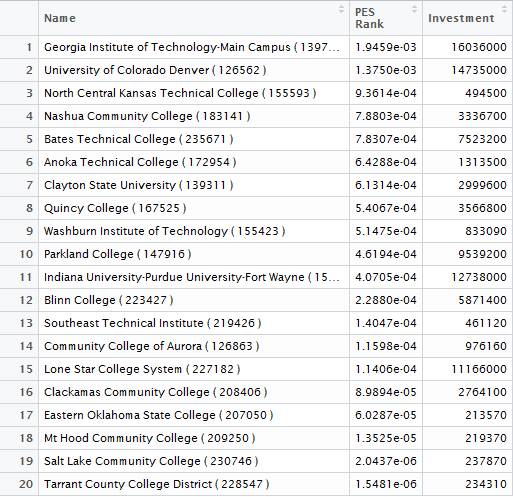
\includegraphics[width=0.7\textwidth]{final.png}
			\caption{Top 20 Schools}
			\label{fig:top20}
		\end{figure}	

\section{Discussion} 
	\subsection{Sensitivity Analysis}
		
		\ \ In order to test model stability, we impose a radius condition to the kNN selection algorithm. The model which was applied in Section 3 used an unrestricted subset of the data. We compute the the mean and standard deviation for each class $i$. Then each value exceeding k from k = 1,..3 standard deviations away was omitted from the data passed to the investment algorithm. The goal is to partition the dataset such that the subset data will have 68\%, 95\%, and 99.7\% of the data.\\

		\ \ With all other variables the same the ROI for each standard deviation(STD) is:
		\begin{enumerate}
		\item STD 1 ROI: 0.0353
		\item STD 2 ROI: 0.0499
		\item STD 3 ROI: 0.0474
		\end{enumerate}

		\ \ All ROI are relatively the same suggesting that the model does well with any size of data input. 

	\subsection{Strengths}
		\begin{itemize}
			\item \textbf{Wide Variety of Variables} The investment strategy looks at all variables provided in the COMAP College Score Card data set. This approach provides a large number of factors to assess an institution's potential for investment rather then the usual ones used by different education foundations. 
		\end{itemize}

	\subsection{Weaknesses}
		\begin{itemize}
		\item \textbf{Institutions with Missing Data} During the early stage process of the data cleaning, schools that did not have data for the two bench mark variables "Incoming Poverty" and "Outgoing Poverty" were removed from the list. It is a possibility that those particular institutions could have skewed the results.
		\item \textbf{Specialized Institutions} Similar to the point above, the data was filtered to remove any institutions that identified as religious-affiliated, race-affiliated, and gender-affiliated. In our first initial tests, many of the specialized institutions were at the top of the ranking systems due to the special nature of their student body. However the trade-off is smaller data set for the investment strategy. 
		\end{itemize}

\section{Extensions}
	\begin{itemize}
		\item \textbf{Determine the correlation between tuition-grants and students' retention rates} A strong underlying of the model is the assumption that students' receiving grants are directly guaranteed to graduate. An in-depth study should be undertaken to put a more precise percentage to the correlation. 

		\item \textbf{Refine the number of observed variables used for the kNN method} Assuming the variables can be fitted to a linear regression model, we can run an R-Squared test. The test results would select the variables that are statistically significant improving the investment strategy. 

		\item \textbf{Run the model on major types} Dependent on the charitable goals of the foundation, the model can be further partitioned to run on schools that focus on different concentrations. For example, select only Law Schools. 

		\item \textbf{Determine the true poverty rate by adjusting for major type} Expanding on the idea above about partitioning into majors, we can refine the adjusted poverty rates. Particular institutions appeal more to lower-income individuals and conversely some universities have predominantly middle-income and above student-bodies. \cite{Carnevale}.
	\end{itemize}

\section{Conclusions}

	\ \ After running our model on the real data, finding the top ranking universities and maximizing the investment of our donations to society. We found the top ranking universities to invest in, as presented in figure 2, and the top ranking universities that are better at taking individuals out of poverty as seen in figures (a),(b), and (c).\\

	\ \ We note that we treated each university as having equal footing in our investment strategy. We saw that this did not matter	as universities with smaller years-to-graduation would still provide a return within 5 years, and each return is only realized after 10 years of graduation.\\
	
	\ \ Our sensitivity analysis on the model, found that it did well with any size of data input after being filtered by the amount of schools that it is allowed to look at. Since the ROI's were relatively close to each other it affirmed our model's results.\\
	
	\ \ However, we do believe that applying each of the ideas outlined in the extensions section of this report would improve the results of the model. Thereby providing the correct schools with the right amount of funds.\\
	
	\ \ Lastly, we would like to point out that while we measured schools as institutions that battle poverty, many may disagree on this view point. If one were to use SAT scores or ACT scores as the variable to determine the ranking of the university, they would still be able to make use of our model, a simple tweaking of the assumption would be required.
\clearpage

\section{Letter to Mr. Alpha Chiang}
Dear Mr. Alpha Chiang, \\

Team \#54301 from the MCM proposes  a concept for return-on-investment (ROI) based on the incoming and outgoing poverty rate of the institution. Given the poverty rate, we rank the institutions and the ROI is calculated by the change in rank (i.e. how much better the institutions work after receiving Goodgrant's donation). 


<<<<<<< HEAD
Overall, we are confident that the proposed investment strategy will exemplify Goodgrant’s fundamental charitable objective. \\

Sincerely,
Team \# 54301
=======
>>>>>>> 7aaef66ef6db70fa7702596e037c20396930e9b0
\newpage



\begin{thebibliography}{10}
	\bibitem{Conkey} Conkey, Christopher 2006. ``Big donations to charity often include spending advice.” \emph{The Wall Street Journal Asia} 
	
	\bibitem{Trom} Trombitas, Kate.  \emph{Financial Stress: An Everyday Reality for College Students}. Inceptia, July 2012. PDF.
	
	\bibitem{dis} US Census Bureau  \emph{The Big Payoff: Educational Attainment and Synthetic Estimates of Work-Life Earnings}. Report, 2006 . PDF. 

	\bibitem{US} ``Using Federal Data To Measure And Improve The Performance Of U.S. Institutions of Higher Education" Sept 2015. \textless https://collegescorecard.ed.gov/assets/UsingFederalDataToMeasureAnd- \\ImprovePerformance.pdf\textgreater.
	
	\bibitem{Hastie} Hastie, Trevor, Robert Tibshirani, and Jerome Friedman. ``Prototype Methods and Nearest-Neighbors". \emph{The Elements of Statistical Learning: Data Mining, Inference, and Prediction.} 2nd ed. New York: Springer, 2009. Print. 
	
	\bibitem{Bill} ``Bill \& Melinda Gates Foundation." \emph{Bill \& Melinda Gates Foundation}. Web. 29 Jan. 2016. 
	
	\bibitem{Grant} ``Grants Database." \emph{Grants Database}. Web. 29 Jan. 2016. $<$https://www.luminafoundation.org/grants-database/strategy/student-financial-supports$>$. 
	
	\bibitem{Winston} Winston, Wayne L. ``Linear Programming."  \emph{Operations Research: Applications and Algorithms}. 4th ed. Belmont, Calif.: Duxbury, 2003. Print.
	
	\bibitem{Carnevale} Carnevale, Anthony, Ban Cheah, and Martin Van Der Werf. \emph{Ranking Your College}. Georgetown University Center on Education and the Workforce, Dec. 2015. PDF.	

	\bibitem{IPEDS} ``IPEDS Data Center." \emph{IPEDS Data Center.} Web. 30 Jan. 2016. \textless https://nces.ed.gov/ipeds/datacenter/DataFiles.aspx\textgreater.

	\bibitem{Wayne} Hanushek, Eric and Margaret Raymond. 2005. ``Does School Accountability Lead to Improved School Performance?” \emph{Journal of Policy Analysis and Management} 24(2): 297-329.
	
	
	
\end{thebibliography}
\end{document}
